\documentclass[final]{article}

\usepackage[preprint]{neurips_2025}

\usepackage[utf8]{inputenc}
\usepackage[T1]{fontenc}
\usepackage{hyperref}
\usepackage{url}
\usepackage{booktabs}
\usepackage{amsfonts}
\usepackage{nicefrac}
\usepackage{microtype}
\usepackage{xcolor}
\usepackage{amsmath}
\usepackage{graphicx}
\usepackage{subcaption}
\usepackage{multirow}
\usepackage{algorithm}
\usepackage{algorithmic}
\usepackage{enumitem}

\graphicspath{{../temporal/figures/}{../enhanced/figures/}{../figures/}{../img/}}

\title{SleepStageNet: Deep Learning for Automated Sleep Stage Classification}

\author{%
  Shrinivas Acharya \\
  % University of Washington \\
  \texttt{acharyas@cs.washington.edu} \\
  \And
  Manish Das \\
  % University of Washington \\
  \texttt{manishuw@cs.washington.edu} \\
  \AND
  Nithin Balachandran \\
  % University of Washington \\
  \texttt{nibalach@cs.washington.edu} \\
  \And
  Regith Lingesh \\
  % University of Washington \\
  \texttt{rlingesh@cs.washington.edu} \\
  \And
  Thangakumar Dhanasekaran \\
  % University of Washington \\
  \texttt{tdhana@cs.washington.edu} \\
}

\begin{document}

\maketitle

\begin{abstract}
Automated sleep staging from raw electroencephalography (EEG) signals promises to reduce the cost and subjectivity of manual polysomnography scoring, which currently requires 2--4 hours of expert effort per overnight recording. We present a systematic comparison of three progressively complex architectures for 5-class sleep stage classification on the Sleep-EDF v1 dataset: (1)~a dual-path multi-scale CNN baseline inspired by DeepSleepNet-Lite, (2)~the same CNN backbone augmented with a two-layer bidirectional LSTM for temporal context modeling, and (3)~a CNN--Conformer hybrid that replaces the recurrent layer with Conformer blocks combining multi-head self-attention and depthwise convolution. All models are evaluated under an identical 20-fold leave-one-subject-out cross-validation protocol. The CNN+BiLSTM model achieves the best performance with 83.9\% accuracy, macro F1 of 0.79, and Cohen's $\kappa$ of 0.778---approaching the lower bound of human inter-scorer agreement ($\kappa \approx 0.75$--$0.85$). Notably, the BiLSTM outperforms the Conformer across all metrics despite having fewer parameters, suggesting that recurrent inductive biases are preferable to attention mechanisms on small sequential EEG datasets. Our results confirm that temporal context modeling is the single most impactful architectural choice for sleep staging, yielding a 3 percentage-point accuracy improvement and a 17.7\% relative gain on the challenging N1 (light sleep) stage.
\end{abstract}

%==============================================================================
\section{Introduction}
%==============================================================================

Sleep disorders affect an estimated 50--70 million Americans, yet diagnosis remains bottlenecked by the manual scoring of polysomnography (PSG) recordings~\cite{Berry2012}. A trained sleep technician examines each 30-second epoch of multi-channel physiological signals and assigns one of five stages---Wake~(W), N1, N2, N3, and REM---according to the American Academy of Sleep Medicine (AASM) guidelines. With 800--1,000 epochs per night, this process takes 2--4 hours per recording, is expensive, and exhibits inter-scorer disagreement with Cohen's $\kappa$ typically in the range of 0.75--0.85~\cite{Rosenberg2013}. Automating this task would reduce cost, improve throughput, and enable scalable sleep monitoring through wearable EEG devices.

Deep learning has demonstrated strong potential for this task. DeepSleepNet~\cite{Supratak2017} introduced a dual-path CNN with a bidirectional LSTM to learn directly from raw single-channel EEG. U-Sleep~\cite{Perslev2021} demonstrated cross-dataset generalization with a U-Net architecture. AttnSleep~\cite{Eldele2021} applied attention mechanisms to capture inter-epoch dependencies, and SleepTransformer~\cite{Phan2022} extended this with epoch-level and sequence-level transformer blocks. Despite these advances, a key question remains understudied: \emph{given the same feature extraction backbone, does recurrent or attention-based temporal modeling yield better performance on small EEG datasets?}

We address this question through a controlled comparison of three architectures sharing a common multi-scale CNN backbone and differing only in their temporal modeling strategy: no temporal modeling (CNN-only baseline), a two-layer BiLSTM, and a three-block Conformer. All three are evaluated under the same 20-fold leave-one-subject-out cross-validation (LOSO-CV) on the Sleep-EDF v1 dataset, isolating the effect of the temporal component.

Our contributions are: (1)~a systematic comparison showing that temporal context is the dominant factor for sleep staging accuracy (+3 pp over baseline); (2)~evidence that BiLSTM outperforms the Conformer on small EEG datasets, achieving $\kappa = 0.778$; and (3)~an analysis of per-class error patterns revealing that temporal models most benefit stages with ambiguous spectral signatures (N1, Wake, REM).

%==============================================================================
\section{Related Work}
%==============================================================================

\paragraph{CNN-based methods.}
DeepSleepNet~\cite{Supratak2017} pioneered a dual-path CNN architecture with small filters ($\sim$0.5\,s) for high-frequency features and large filters ($\sim$4\,s) for slow-wave patterns, followed by a BiLSTM for sequence modeling. DeepSleepNet-Lite~\cite{Fiorillo2019} simplified this design for lower computational cost while preserving the dual-path concept. Our baseline adopts this dual-path philosophy with parallel CNN paths operating at different temporal resolutions.

\paragraph{Temporal and attention-based methods.}
Recurrent neural networks, particularly LSTMs~\cite{Hochreiter1997} and their bidirectional variants~\cite{Schuster1997}, have been widely used to model sleep stage transitions. More recently, attention mechanisms~\cite{Vaswani2017} have been applied: AttnSleep~\cite{Eldele2021} uses multi-head attention over CNN features, and SleepTransformer~\cite{Phan2022} employs epoch-level and sequence-level transformer blocks. The Conformer architecture~\cite{Gulati2020}, originally developed for speech recognition, combines self-attention with depthwise convolution in a Macaron-style block, capturing both global and local patterns. We adapt the Conformer for EEG epoch sequences and compare it against a BiLSTM under identical conditions.

\paragraph{Training techniques for imbalanced EEG data.}
Class imbalance is pervasive in sleep staging (N1 constitutes only $\sim$7\% of epochs). Focal loss~\cite{Lin2017} down-weights easy examples to focus learning on hard cases. Mixup~\cite{Zhang2018} interpolates training pairs for smoother decision boundaries. Label smoothing~\cite{Berry2012} softens one-hot targets to reduce overconfidence. We employ these techniques in combination with a three-stage training pipeline and cosine annealing with warmup~\cite{Loshchilov2017}.

%==============================================================================
\section{Dataset}
%==============================================================================

We use the \textbf{Sleep-EDF v1} dataset from PhysioNet~\cite{SleepEDF2018, Goldberger2000}, containing 39 whole-night PSG recordings from 20 healthy subjects. Each recording provides the Fpz-Cz EEG channel at 100\,Hz, with expert annotations assigning each 30-second epoch (3,000 samples) to one of five AASM sleep stages~\cite{Berry2012}.

The dataset contains 42,308 epochs with severe class imbalance (Figure~\ref{fig:class_dist}): N2 dominates at 42.1\% of all epochs, while the transitional N1 stage comprises only 6.6\%, creating a 6.4:1 imbalance ratio. This imbalance makes accuracy misleading---a trivial majority-class classifier achieves 42\%---and motivates our use of macro F1 as the primary evaluation metric.

\begin{figure}[t]
  \centering
  
\includegraphics[width=0.65\columnwidth]{class_distribution.png}
  \caption{Sleep stage distribution in Sleep-EDF v1 (42,308 epochs from 39 recordings). N2 dominates at 42.1\% while the transitional N1 stage comprises only 6.6\% of epochs.}
  \label{fig:class_dist}
\end{figure}

%==============================================================================
\section{Methods}
%==============================================================================

We develop three architectures of increasing complexity. All share a multi-scale CNN feature extractor; they differ in how (or whether) temporal context across epochs is modeled.

%--------------------------------------
\subsection{Multi-Scale CNN Backbone}
\label{sec:cnn_backbone}
%--------------------------------------

Inspired by DeepSleepNet~\cite{Supratak2017} and DeepSleepNet-Lite~\cite{Fiorillo2019}, our CNN uses two parallel paths operating at different temporal resolutions (Figure~\ref{fig:architecture}):

\textbf{Path~A (fine-grained, $\sim$0.5\,s resolution)} captures high-frequency features such as sleep spindles (12--14\,Hz) and K-complexes:
Conv1d($C_{\text{in}} \!\to\! 32$, $k\!=\!50$, $s\!=\!6$) $\to$ BN $\to$ ReLU $\to$ MaxPool(8) $\to$ three Conv1d($\to$64, $k\!=\!8$) blocks each with BN and ReLU $\to$ MaxPool(4) $\to$ AdaptiveAvgPool(1), producing a 64-dimensional vector.

\textbf{Path~B (coarse, $\sim$4\,s resolution)} captures slow-wave activity (0.5--2\,Hz):
Conv1d($C_{\text{in}} \!\to\! 32$, $k\!=\!400$, $s\!=\!50$) $\to$ BN $\to$ ReLU $\to$ MaxPool(4) $\to$ three Conv1d($\to$64, $k\!=\!6$) blocks $\to$ MaxPool(2) $\to$ AdaptiveAvgPool(1), producing a 64-dimensional vector.

The two 64-dim outputs are concatenated, passed through dropout (0.5) and a linear projection to a 128-dimensional feature vector. This backbone is shared across the temporal models (BiLSTM and Conformer) and applied independently to each epoch in a sequence.

\begin{figure}[t]
  \centering
  \includegraphics[width=0.85\columnwidth]{deepsleepnet-lite.png}
  \caption{Dual-path CNN architecture inspired by DeepSleepNet-Lite~\cite{Fiorillo2019}. Path~1 uses small filters to capture high-frequency sleep spindles; Path~2 uses large filters for slow-wave detection. Our PyTorch re-implementation follows the same topology with channel counts of 32/64.}
  \label{fig:architecture}
\end{figure}

%--------------------------------------
\subsection{Model~1: CNN-Only Baseline}
%--------------------------------------

The baseline model concatenates three consecutive 30-second epochs into a 90-second input window (9,000 samples at 100\,Hz) and passes it through a dual-path CNN similar to the backbone described above, but implemented in TensorFlow following the original DeepSleepNet-Lite design~\cite{Fiorillo2019}. This model uses 64/128 channel filters (rather than 32/64) without adaptive pooling, resulting in $\sim$648K parameters. It classifies each center epoch using only the local context provided by the concatenated window.

Training uses Adam (lr $= 10^{-4}$), batch size 100, 100 epochs with early stopping (patience 50), and minority-class oversampling to handle imbalance.

%--------------------------------------
\subsection{Model~2: CNN + BiLSTM}
%--------------------------------------

Rather than concatenating epochs into a single window, this model processes each epoch independently through the shared multi-scale CNN backbone (Section~\ref{sec:cnn_backbone}) to obtain a 128-dimensional feature vector per epoch. A sequence of $L = 11$ consecutive epoch features ($\pm$5 epochs of temporal context) is then passed to a \textbf{two-layer bidirectional LSTM}~\cite{Hochreiter1997, Schuster1997} with hidden size 128 per direction, producing a 256-dimensional output per timestep. The center epoch's output (position $\lfloor L/2 \rfloor = 5$) is extracted and classified through dropout (0.3) and a linear layer to 5 classes.

This design explicitly models the temporal structure of sleep: the BiLSTM can learn that N1 typically occurs as a transition between Wake and N2, or that REM epochs cluster in cycles. The model has $\sim$851K parameters.

%--------------------------------------
\subsection{Model~3: CNN + Conformer}
%--------------------------------------

This model replaces the BiLSTM with \textbf{three Conformer blocks}~\cite{Gulati2020}, each using the Macaron-style architecture:

\begin{enumerate}[nosep, leftmargin=*]
  \item \textbf{Half-step FFN}: LayerNorm $\to$ Linear(128$\to$512) $\to$ GELU $\to$ Dropout $\to$ Linear(512$\to$128) $\to$ 0.5$\times$ residual
  \item \textbf{Multi-head self-attention}: LayerNorm $\to$ MHSA (4 heads, $d_k = 32$) $\to$ Dropout $\to$ residual
  \item \textbf{Convolution module}: LayerNorm $\to$ Pointwise Conv (128$\to$256) $\to$ GLU $\to$ Depthwise Conv ($k\!=\!7$, groups=128) $\to$ BN $\to$ GELU $\to$ Pointwise Conv (128$\to$128) $\to$ Dropout $\to$ residual
  \item \textbf{Half-step FFN}: Same as step 1, with 0.5$\times$ residual
  \item \textbf{Final LayerNorm}
\end{enumerate}

Learnable positional encoding is added before the Conformer blocks, as it outperforms fixed sinusoidal encoding for short sequences ($L = 11$). The center epoch output is classified identically to the BiLSTM model. The Conformer uses focal loss~\cite{Lin2017} with $\gamma = 1.5$ instead of cross-entropy, to focus learning on hard examples such as N1. The model has $\sim$1.34M parameters.

%--------------------------------------
\subsection{Training Strategy}
\label{sec:training}
%--------------------------------------

Both the BiLSTM and Conformer models use a \textbf{three-stage training pipeline} to avoid the instability of jointly training the CNN and temporal layers from scratch:

\begin{algorithm}[t]
\caption{Three-Stage Training Pipeline}
\label{alg:training}
\begin{algorithmic}[1]
\STATE \textbf{Stage 1: CNN Pre-training.} Train the multi-scale CNN as a single-epoch classifier ($L=1$) using AdamW (lr $= 10^{-3}$) for up to 50 epochs with early stopping on validation macro F1.
\STATE Save pre-trained CNN weights $\theta_{\text{CNN}}^{*}$.
\STATE \textbf{Stage 2: Temporal Layer Training.} Freeze $\theta_{\text{CNN}}^{*}$. Train only the temporal layers (BiLSTM or Conformer) on sequences of $L = 11$ epochs using AdamW with model-specific learning rates for up to 50 epochs.
\STATE \textbf{Stage 3: End-to-End Fine-tuning.} Unfreeze all parameters. Fine-tune with 10$\times$ reduced learning rate for up to 30 epochs. Mixup $\alpha$ reduced by 50\%.
\end{algorithmic}
\end{algorithm}

\paragraph{Regularization.} We employ several complementary techniques: (a)~\textbf{Mixup}~\cite{Zhang2018} with $\alpha = 0.1$ applied to 50\% of training batches (BiLSTM and Conformer); (b)~\textbf{label smoothing} of 0.05 across all models; (c)~\textbf{EEG-specific data augmentation} including time shift ($\pm$50 samples), amplitude scaling ($\pm$10\%), and Gaussian noise; (d)~\textbf{cosine annealing with linear warmup}~\cite{Loshchilov2017} (3-epoch warmup); and (e)~\textbf{gradient clipping} (max norm 1.0) for the temporal stages to prevent LSTM gradient explosion. Class imbalance is addressed through inverse class-frequency weighting via \texttt{compute\_class\_weight('balanced')}.

Table~\ref{tab:hyperparams} summarizes the key hyperparameters for each model.

\begin{table}[t]
\caption{Hyperparameter comparison across the three models.}
\label{tab:hyperparams}
\centering
\small
\begin{tabular}{lccc}
\toprule
\textbf{Hyperparameter} & \textbf{Baseline} & \textbf{CNN+BiLSTM} & \textbf{CNN+Conformer} \\
\midrule
Framework        & TensorFlow   & PyTorch     & PyTorch \\
Sequence length  & 3 (concat)   & 11          & 11 \\
Batch size       & 100          & 32          & 32 \\
Learning rate    & $10^{-4}$    & $5 \times 10^{-4}$ & $3 \times 10^{-4}$ \\
Optimizer        & Adam         & AdamW       & AdamW \\
Loss function    & Cross-entropy & Cross-entropy & Focal ($\gamma\!=\!1.5$) \\
Mixup $\alpha$   & ---          & 0.1         & 0.1 \\
Label smoothing  & 0            & 0.05        & 0.05 \\
Patience         & 50           & 15          & 20 \\
Parameters       & $\sim$648K   & $\sim$851K  & $\sim$1.34M \\
\bottomrule
\end{tabular}
\end{table}

%==============================================================================
\section{Experimental Setup}
%==============================================================================

\paragraph{Evaluation protocol.}
We use 20-fold leave-one-subject-out cross-validation (LOSO-CV): in each fold, one subject's recordings are held out for testing, with the remaining 19 subjects split into training (15) and validation (4) sets. Sequences never cross recording boundaries, preventing data leakage.

\paragraph{Metrics.}
We report overall accuracy, \textbf{macro F1} (primary metric---treats all 5 classes equally, penalizing poor N1 performance), Cohen's $\kappa$~\cite{Cohen1960} (the clinical standard, correcting for chance agreement), and per-class F1 scores. For the temporal models we report mean $\pm$ standard deviation across the 20 folds.

\paragraph{Implementation.}
The baseline is implemented in TensorFlow/Keras; the CNN+BiLSTM and Conformer models in PyTorch. All experiments run on Google Colab with NVIDIA T4 GPUs.

%==============================================================================
\section{Results}
%==============================================================================

%--------------------------------------
\subsection{Overall Comparison}
%--------------------------------------

Table~\ref{tab:main_results} presents the main results. Both temporal models significantly improve over the CNN-only baseline across all metrics. The CNN+BiLSTM achieves the best overall performance with 83.9\% accuracy, macro F1 of 0.79, and $\kappa = 0.778$, outperforming the more complex Conformer on every metric despite having 37\% fewer parameters in total (851K vs.\ 1.34M).

\begin{table}[t]
\caption{Overall performance comparison. $\star$ indicates the best model. The baseline reports single aggregate values from 20-fold pooled predictions; temporal models report mean $\pm$ std across 20 folds.}
\label{tab:main_results}
\centering
\small
\begin{tabular}{lcccc}
\toprule
\textbf{Model} & \textbf{Accuracy} & \textbf{Macro F1} & \textbf{Cohen's $\kappa$} & \textbf{N1 F1} \\
\midrule
Baseline (CNN)           & 80.9\%                  & 0.753              & 0.740               & 0.441 \\
CNN+BiLSTM $\star$       & 83.9\% $\pm$ 6.5\%     & 0.79 $\pm$ 0.067   & 0.778 $\pm$ 0.091   & 0.519 \\
CNN+Conformer            & 83.0\% $\pm$ 7.3\%     & 0.78 $\pm$ 0.07    & 0.768 $\pm$ 0.10    & 0.500 \\
\bottomrule
\end{tabular}
\end{table}

The improvement from baseline to the best temporal model is consistent: +3.0 pp accuracy, +0.037 macro F1, and +0.038 $\kappa$. This confirms that temporal context modeling is the single most impactful architectural choice.

%--------------------------------------
\subsection{Per-Class Analysis}
%--------------------------------------

Table~\ref{tab:per_class} shows the per-class F1 scores for all three models. The temporal models yield the largest improvements on stages that benefit most from transition context: Wake (+7.9 pp F1 for BiLSTM), REM (+6.1 pp), and the challenging N1 (+7.8 pp). N2 and N3 are already well-classified by the baseline (F1 $> 0.85$) and show only marginal gains.

\begin{table}[t]
\caption{Per-class F1 scores across all three models. Bold indicates the best per-class result. The improvement column ($\Delta$) shows the BiLSTM gain over the baseline.}
\label{tab:per_class}
\centering
\small
\begin{tabular}{lccccc}
\toprule
\textbf{Stage} & \textbf{Baseline} & \textbf{CNN+BiLSTM} & \textbf{CNN+Conformer} & $\boldsymbol{\Delta}$ \\
\midrule
Wake  & 0.802 & \textbf{0.881} & 0.870 & +0.079 \\
N1    & 0.441 & \textbf{0.519} & 0.500 & +0.078 \\
N2    & 0.865 & \textbf{0.869} & \textbf{0.869} & +0.004 \\
N3    & 0.859 & \textbf{0.877} & 0.874 & +0.018 \\
REM   & 0.795 & \textbf{0.856} & 0.834 & +0.061 \\
\bottomrule
\end{tabular}
\end{table}

N1 remains the bottleneck for all models: the best F1 of 0.519 (BiLSTM) represents a 17.7\% relative improvement over the baseline but is still far below other stages. From the baseline confusion matrix, N1 is confused with Wake (14\% of N1 epochs), N2 (22\%), and REM (15\%)---its EEG signature overlaps all three neighboring stages. Temporal context helps because the model can use transition likelihood: N1 rarely follows N3 directly, and the typical N1 pattern involves a transition from Wake toward N2 or from N2 toward REM.

Figure~\ref{fig:per_class_f1} provides a visual comparison of per-class F1 scores between the CNN+BiLSTM and Conformer models.

\begin{figure}[t]
  \centering
  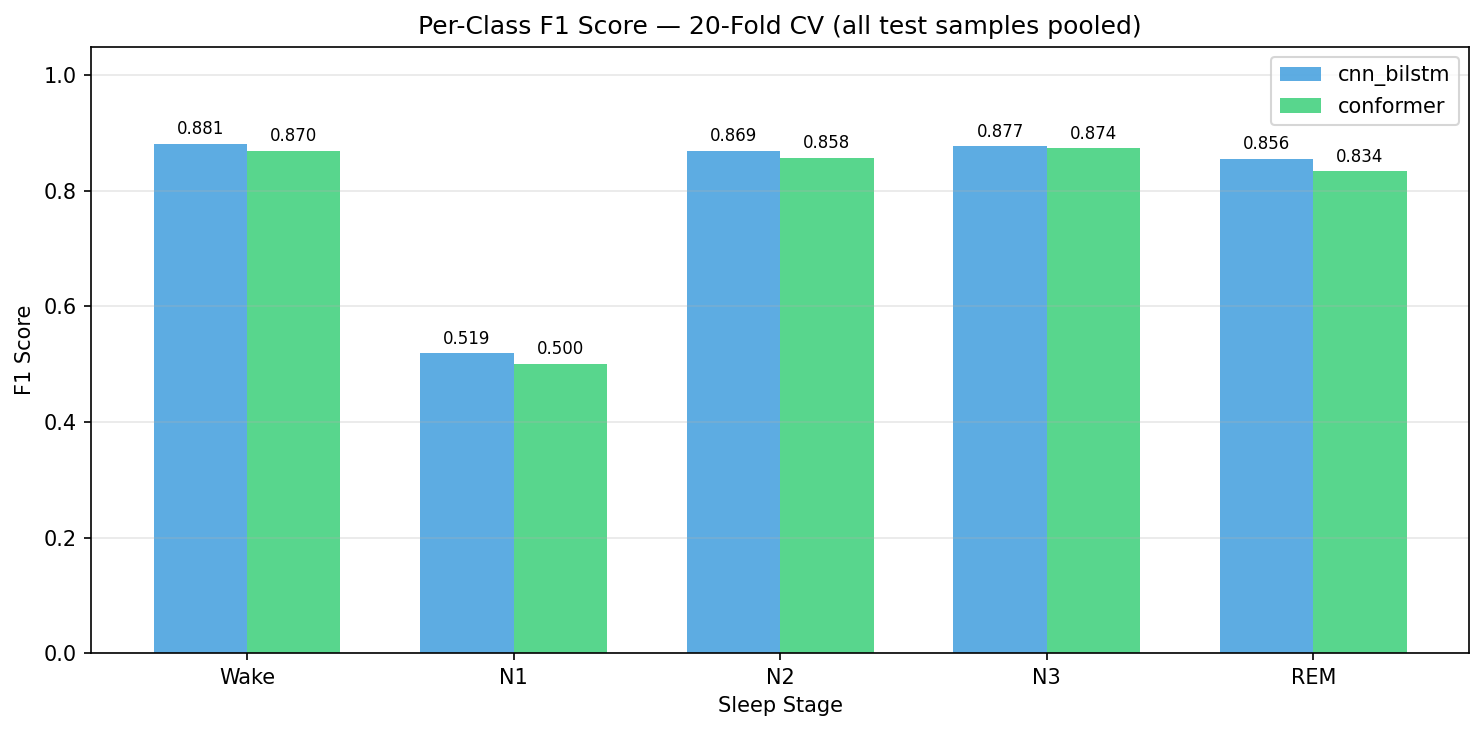
\includegraphics[width=0.75\columnwidth]{cv20_per_class_f1.png}
  \caption{Per-class F1 score comparison between CNN+BiLSTM and CNN+Conformer across 20-fold LOSO-CV. The BiLSTM leads on all stages except N2 (tied).}
  \label{fig:per_class_f1}
\end{figure}

%--------------------------------------
\subsection{Cross-Validation Stability}
%--------------------------------------

Figure~\ref{fig:boxplots} shows the distribution of metrics across the 20 LOSO-CV folds. Both temporal models exhibit high inter-subject variance (std 6.5--7.3\% for accuracy), reflecting the inherent diversity of individual sleep architectures. The BiLSTM shows slightly tighter distributions (lower standard deviation) than the Conformer on all metrics. Fold~11 is a consistent outlier for both models ($\sim$62--64\% accuracy), suggesting that this subject's sleep patterns are atypical.

\begin{figure}[t]
  \centering
  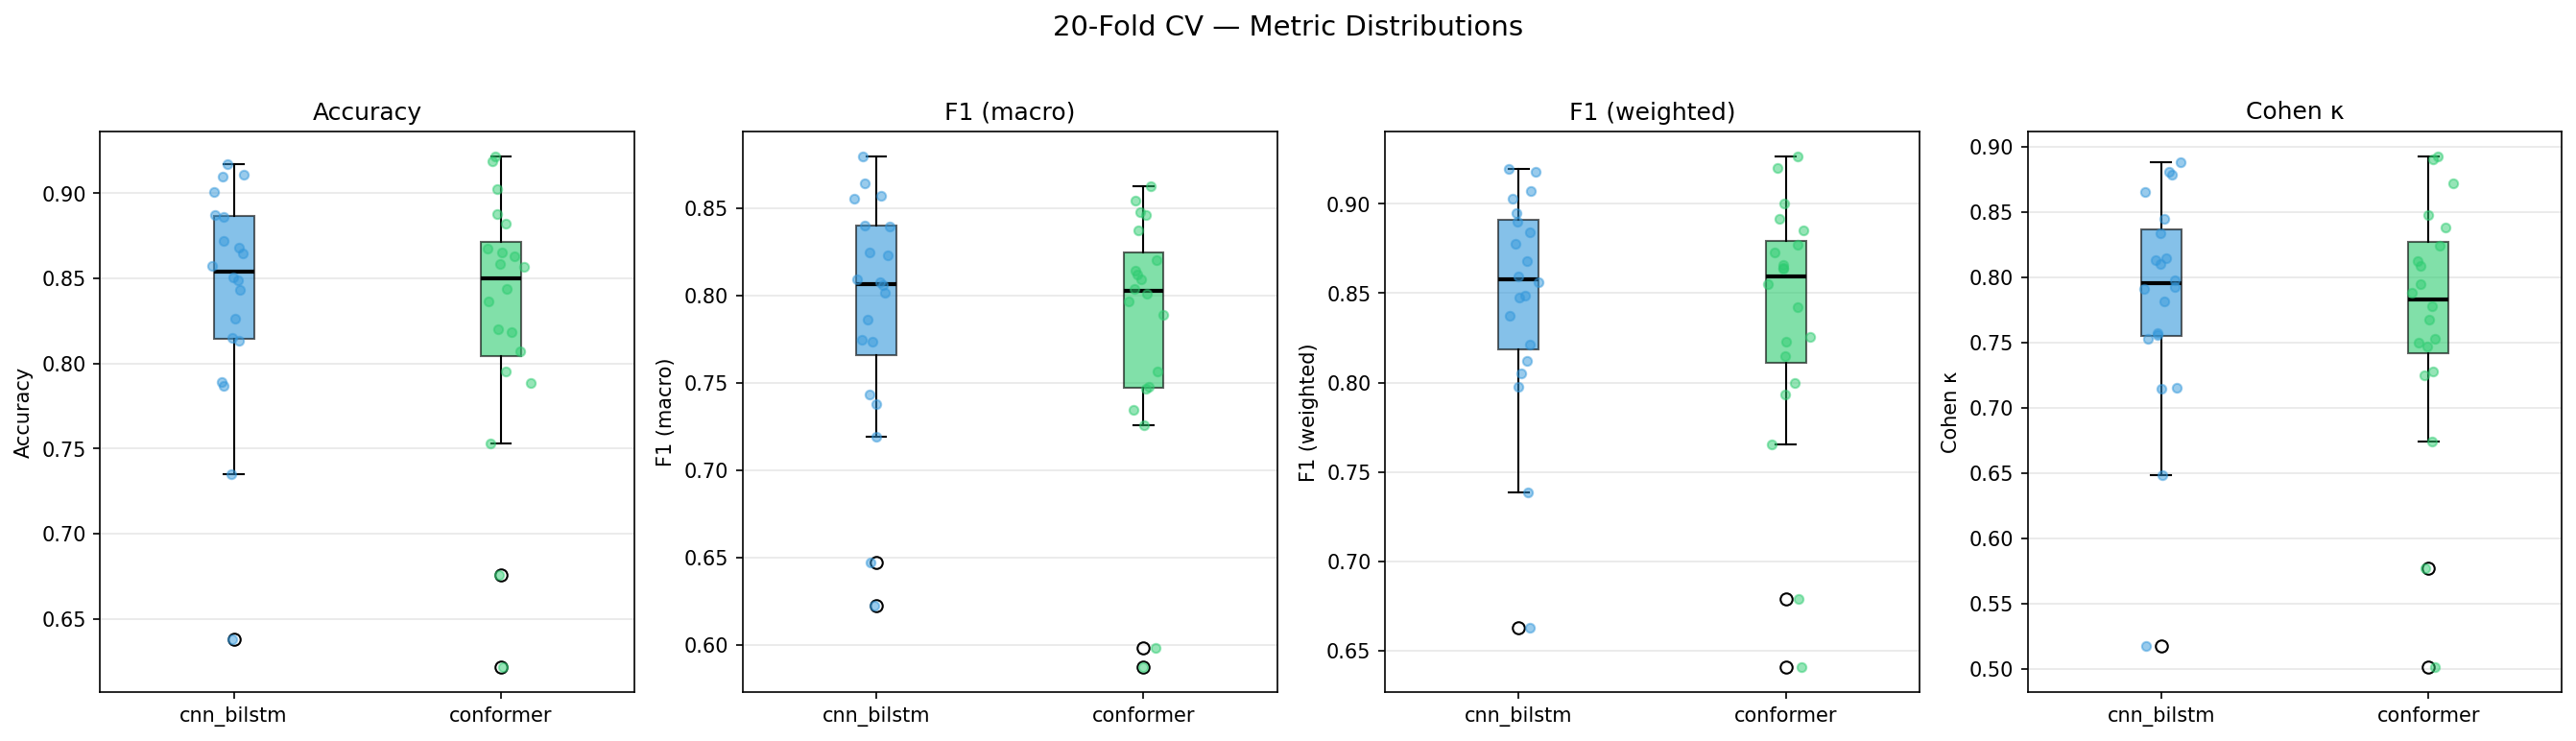
\includegraphics[width=0.85\columnwidth]{cv20_boxplots.png}
  \caption{Distribution of evaluation metrics across 20 LOSO-CV folds for CNN+BiLSTM and Conformer. The BiLSTM exhibits tighter distributions on all metrics.}
  \label{fig:boxplots}
\end{figure}

Figure~\ref{fig:confusion} presents the pooled confusion matrices. The temporal models show substantially reduced off-diagonal mass in the Wake and REM rows compared to the baseline, confirming that temporal context resolves many Wake$\leftrightarrow$N1 and N1$\leftrightarrow$REM confusions.

\begin{figure}[t]
  \centering
  \begin{subfigure}[b]{0.48\textwidth}
    \centering
    
\includegraphics[width=\textwidth]{../figures/confusion_matrices.png}
    \caption{Baseline (CNN-only)}
  \end{subfigure}
  \hfill
  \begin{subfigure}[b]{0.48\textwidth}
    \centering
    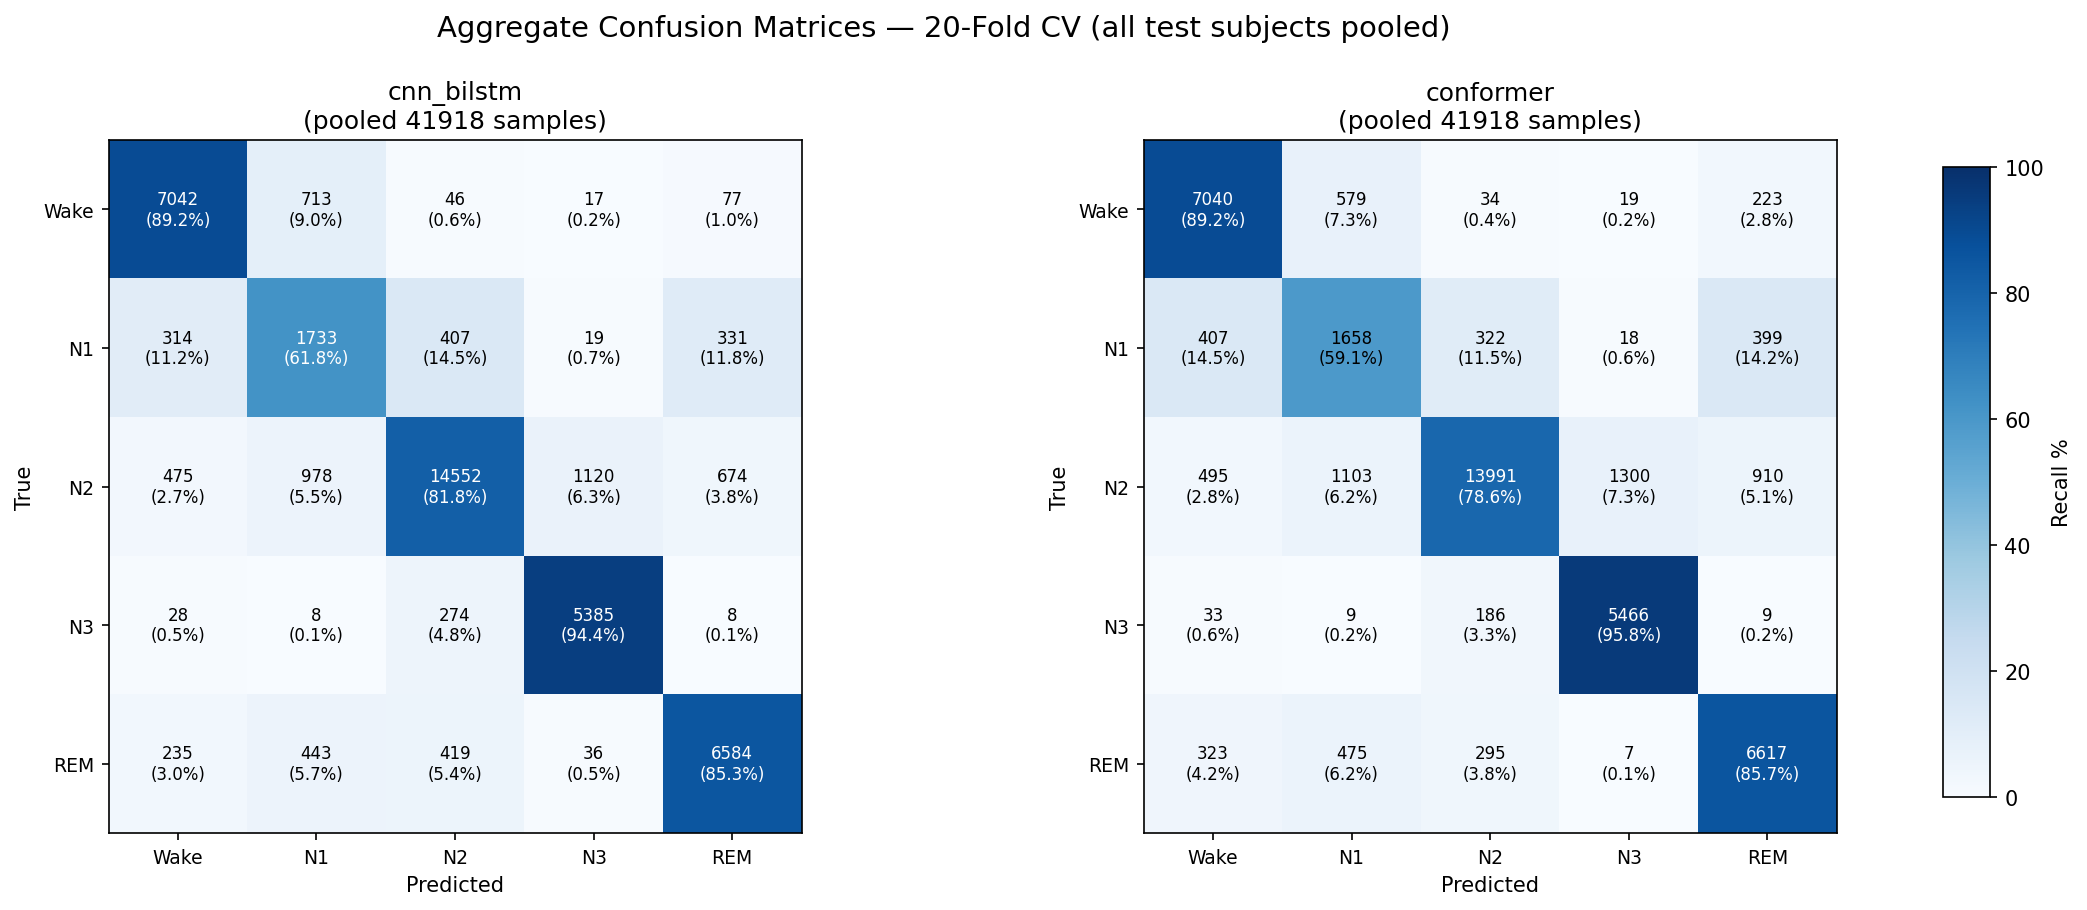
\includegraphics[width=\textwidth]{cv20_confusion_matrices.png}
    \caption{CNN+BiLSTM and CNN+Conformer}
  \end{subfigure}
  \caption{Pooled confusion matrices across all 20 folds. (a)~Baseline shows heavy N1 confusion with Wake and N2. (b)~Temporal models substantially reduce these off-diagonal errors.}
  \label{fig:confusion}
\end{figure}

%--------------------------------------
\subsection{Clinical Context}
%--------------------------------------

Cohen's $\kappa = 0.778$ for the CNN+BiLSTM places it at the lower bound of human inter-scorer agreement ($\kappa \approx 0.75$--$0.85$)~\cite{Rosenberg2013}. The 3 pp accuracy gap between baseline and temporal models translates to approximately 1,200 fewer misclassified epochs across the full test set. The single-channel EEG requirement (Fpz-Cz only) makes this approach applicable to consumer-grade wearable devices, though the N1 F1 of 0.519 would need further improvement for diagnostic applications where detecting sleep onset is critical.

%==============================================================================
\section{Discussion}
%==============================================================================

%--------------------------------------
\subsection{Why Does BiLSTM Outperform Conformer?}
%--------------------------------------

The CNN+BiLSTM outperforms the more parameter-rich Conformer across all metrics. We identify four contributing factors:

\textbf{Inductive bias.} The BiLSTM has a strong sequential inductive bias---it processes epochs in temporal order, naturally encoding proximity and direction. Sleep stage transitions are inherently sequential (one does not jump from N3 to REM without passing through lighter stages). The Conformer's self-attention treats all positions as equally accessible and must learn this sequential structure purely from data.

\textbf{Dataset size.} With only 20 subjects and $\sim$42K epochs, the Conformer's larger parameter count (1.34M vs.\ 851K) may lead to overfitting. Attention mechanisms are known to be data-hungry, and 42K training epochs may be insufficient for the Conformer to realize its theoretical advantages over recurrence.

\textbf{Sequence length.} At $L = 11$, the sequence is short enough that the BiLSTM can model dependencies across the full window without suffering from vanishing gradients. Self-attention's advantage---direct pairwise connections between distant positions---is less pronounced when all positions are already within the LSTM's effective memory horizon.

\textbf{Loss function confound.} The Conformer used focal loss ($\gamma = 1.5$) while the BiLSTM used standard cross-entropy. Although focal loss was intended to improve N1 classification, it may have suboptimally reduced the learning signal for well-classified stages, slightly hurting overall calibration.

%--------------------------------------
\subsection{The N1 Problem}
%--------------------------------------

N1 (light sleep) remains the primary bottleneck across all models, with a best F1 of 0.519. This difficulty is not unique to our approach---it reflects fundamental properties of the N1 stage:

\begin{itemize}[nosep, leftmargin=*]
  \item \textbf{Spectral ambiguity:} N1's EEG morphology overlaps with Wake (theta activity in both), N2 (vertex sharp waves resemble K-complexes), and REM (low-amplitude mixed-frequency patterns in both).
  \item \textbf{Brevity:} N1 is a transitional stage lasting only 1--7 minutes, producing few contiguous epochs for learning. It accounts for just 6.6\% of all epochs.
  \item \textbf{Human disagreement:} Even trained scorers exhibit lower inter-rater reliability on N1 than on other stages~\cite{Rosenberg2013}, suggesting an intrinsic limit to automated N1 classification from single-channel EEG.
\end{itemize}

Despite these challenges, temporal context provides a meaningful boost (+17.7\% relative F1). The BiLSTM can leverage transition patterns---e.g., recognizing that an ambiguous epoch between a sequence of Wake epochs and the onset of N2 is likely N1---but cannot fully resolve the underlying spectral ambiguity.

%==============================================================================
\section{Limitations and Future Work}
%==============================================================================

\paragraph{Limitations.}
Our study has several limitations: (1)~\textbf{Single EEG channel}---human scorers use electrooculography (EOG) and electromyography (EMG) in addition to EEG, providing complementary information our models lack; (2)~\textbf{Small dataset}---20 subjects limits generalization claims, and no external validation on larger datasets (e.g., SHHS, MASS) was performed; (3)~\textbf{High subject variance}---some folds achieve $<$65\% accuracy, indicating that certain individuals' sleep patterns are poorly captured by a one-size-fits-all model; (4)~\textbf{No statistical significance testing}---paired tests across folds between BiLSTM and Conformer would strengthen the comparison; (5)~\textbf{Framework confound}---the baseline uses TensorFlow while temporal models use PyTorch, introducing a minor implementation variable.

\paragraph{Future directions.}
Several avenues could address these limitations: (1)~\textbf{Multi-modal inputs}: adding EOG and EMG channels to match clinical practice; (2)~\textbf{Pre-training on larger corpora}: training on SHHS (5,000+ subjects) then fine-tuning on Sleep-EDF, which may also unlock the Conformer's capacity advantage; (3)~\textbf{Subject-adaptive fine-tuning}: few-shot personalization or meta-learning (MAML) to reduce inter-subject variance; (4)~\textbf{N1-targeted strategies}: stage-conditional focal loss with higher $\gamma$ for N1, or synthetic N1 generation via EEG data augmentation; and (5)~\textbf{Uncertainty quantification}: MC-Dropout confidence estimates for flagging low-confidence epochs in clinical deployment.

%==============================================================================
\section{Conclusion}
%==============================================================================

We presented a systematic comparison of three architectures for automated sleep stage classification, sharing a common multi-scale CNN backbone and differing in temporal modeling. Our results demonstrate that temporal context modeling is the dominant factor for performance, yielding a 3 pp accuracy improvement and 17.7\% relative N1 F1 gain over the CNN-only baseline. The CNN+BiLSTM model achieves $\kappa = 0.778$, approaching the lower bound of human inter-scorer agreement, and outperforms the more complex Conformer---suggesting that recurrent inductive biases are preferable to attention mechanisms on small sequential EEG datasets with $\sim$42K training examples. As wearable EEG devices become more prevalent, lightweight models that operate on single-channel input while achieving near-expert-level agreement will be essential for scalable sleep medicine.

\bibliographystyle{plain}
\bibliography{references}

\end{document}
